\chapter[Análise de desempenho]
{An\'alise de desempenho}

Uma vez concretizada a infraestrutura e o \emph{deploy} da aplicação, é necessário analisar o desempenho do serviço, recorrendo a métodos de geração de dados, a rotinas de testes e iterações de modo a obter resultados que possam fundamentar medidas a tomar.

O objectivo da análise de desempenho é perceber até que ponto o serviço escala sem ocorrerem problemas e quais são os \emph{bottlenecks}, caso existam de uma forma explícita, que contribuem para o contrário.

\section{Povoação da base de dados}

Por forma a incluir alguma carga de registos no serviço, tais como utilizadores, círculos, despesas e pagamentos, optou-se por implementar um \emph{script} na linguagem \emph{PHP}.


A linha de pensamento seguida foi:
\begin{itemize}
	\item \textbf{Adicionar utilizadores no sistema} \\
		\indent A adição de utilizadores é necessária, visto que todo o resto do procedimento de geração de dados se torna dependente destes. Para obter a lista de utilizadores, recorreu-se à \emph{API} do \emph{www.randomuser.me}. Para registar utilizadores no sistema, usou-se o seguinte comando:
		\begin{verbatim}
			php seedRegisteredUser.php <quantity>
		\end{verbatim}

	\item \textbf{Adicionar círculos de utilizadores} \\
		\indent Tendo em conta que, no sistema, os círculos são os pontos de encontro de utilizadores, torna-se essencial gerar alguns de modo a que possam interagir através da adição de despesas e os respetivos pagamentos.
		\begin{verbatim}
			php seedCircle.php <quantity>
		\end{verbatim}

	\item \textbf{Adicionar despesas aos círculos} \\
		\indent Tendo em conta que, no sistema, os círculos são os pontos de encontro de utilizadores, torna-se essencial gerar alguns de modo a que possam interagir através da adição de despesas e os respetivos pagamentos.
		\begin{verbatim}
			php seedExpense.php <quantity_per_circle>
		\end{verbatim}

	\item \textbf{Adicionar pagamentos de despesas} \\
		\indent Para simular algum estado com algumas alterações, foram simulados pagamentos de despesa, de modo a verificar diferentes estados da aplicação.
		\begin{verbatim}
			php seedPayment.php
		\end{verbatim}
\end{itemize}

Note que os estados intermédios de cada comando são recolhidos do estado da base de dados e guardados localmente, no formato \emph{JSON}.

Desta forma, depois de inseridos os estados, pode dar-se início à rotina de recolha de dados sobre o comportamento do sistema face às cargas a que é sujeito, que será explicada de seguida.

\section{Rotina}

Como se referiu anteriormente, foi seguida uma rotina para a execução do \emph{benchmark}, que consiste na tomada de vários passos para obter os resultados do desempenho do sistema. Antes de iniciar a rotina, é reposto o estado inicial da base de dados, ou seja, o estado final após a geração de dados.

Fez-se uso da ferramenta \emph{Apache Bench}, cujo objectivo, como o nome indica, é efetuar um determinado número de pedidos ao \emph{URL} que lhe é passado, neste caso o da \emph{dashboard} do utilizador, onde o custo de carregamento de todos os \emph{widgets} nela incluídos se torna interessante de pôr em questão. Os passos tomados na rotina foram os seguintes:

\begin{itemize}
	\item Execução de um aquecimento prévio da base de dados;
	\item Execução do \emph{Apache Bench} para 500 pedidos com 8 clientes concorrentes;
	\item Execução do \emph{Apache Bench} para 500 pedidos com 16 clientes concorrentes;
	\item Execução do \emph{Apache Bench} para 500 pedidos com 32 clientes concorrentes;
	\item Geração de gráficos.
\end{itemize}

\section{Ambiente de teste}

Antes de iniciar os testes, foi preparado o seguinte ambiente de teste:

\begin{itemize}
	\item \emph{\emph{Router}} por cabo com \textit{~1.3ms} de latência
	\item \textbf{Quatro computadores:}
		\begin{itemize}
			\item \textbf{MacBook Pro 13" Late 2013}
				\begin{itemize}
					\item Core i5 (I5-4258U) 2.6GHz
					\item 16GB RAM
					\item 256GB SSD
					\item \textbf{Suporta:} \emph{Web Servers, Application Servers}
				\end{itemize}

			\item \textbf{MacBook Pro 13" Retina 2012}
				\begin{itemize}
					\item Core i5 (I5-3210M) 2.5GHz
					\item 8GB RAM
					\item 128GB SSD
					\item \textbf{Suporta:} \emph{Storage, Service Cluster}
				\end{itemize}

			\item \textbf{MacBook Air 13" 2012}
				\begin{itemize}
					\item Core i5 (I5-3427U) 1.8GHz
					\item 4GB RAM
					\item 128GB SSD
					\item \textbf{Suporta:} \emph{Application Cache Servers, Load Balancers}
				\end{itemize}

			\item \textbf{MacBook Pro 15" (Unibody)}
				\begin{itemize}
					\item Core 2 Duo (T9400) 2.53 GHz
					\item 4GB RAM
					\item 256GB SSD
					\item \textbf{Suporta:} \emph{Apache Bench, Load Balancers}
				\end{itemize}
		\end{itemize}
\end{itemize}

As diferenças a nível de características podem influenciar os resultados dos testes. Na secção seguinte, serão discutidos os resultados obtidos.

\section{Iterações}

Por forma a perceber qual o comportamento da aplicação na infraestrutura que a suporta, aplicou-se o \emph{benchmark} a várias iterações, alterando o número de \emph{Application Servers}, usufruindo da capacidade de escalar horizontalmente esta componente.

Inicialmente procedeu-se a uma otimização da base de dados, como será visto de seguida.

\subsection{Otimização da Base de Dados}

A base de dados é gerada durante o \emph{deployment} da aplicação no servidor aplicacional. Como o \emph{Hibernate} não tem conhecimento da aplicação, não é da responsabilidade do mesmo adicionar índices nem otimizar a base de dados.

A figura seguinte relata os resultados pré-otimização e pós-otimização com dois servidores aplicacionais.

\begin{figure}[H]
\centerline{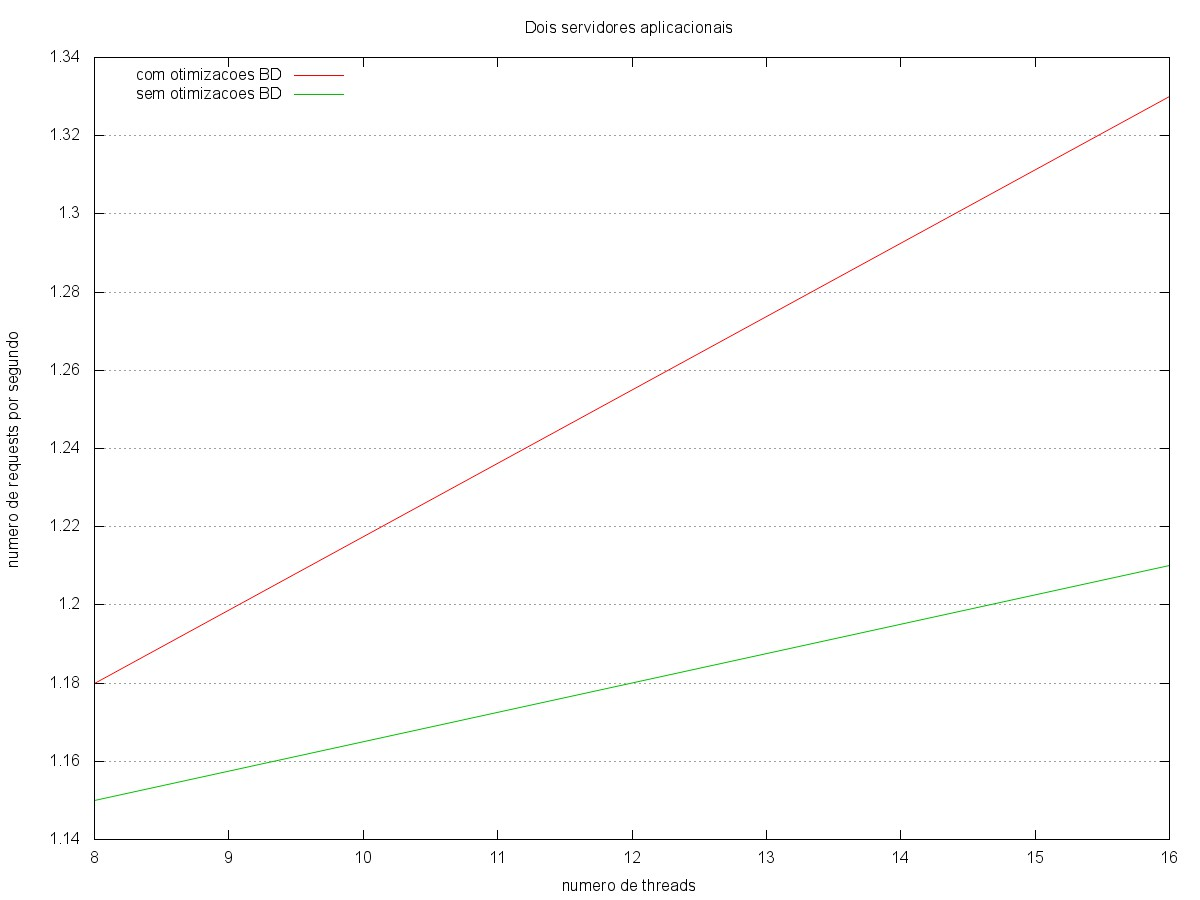
\includegraphics[width=1\textwidth]{images/benchmark/optimization}}
\label{fig:optimization}
\caption{Resultados obtidos antes e depois da otimização}
\end{figure}

Repare que, com otimização, a situação não é tão grave como sem otimização. Para atingir este objetivo, atentou-se nas \emph{queries} efetuadas com mais de \emph{10ms} de tempo de execução, adicionaram-se índices e ordenaram-se algumas tabelas de acordo com alguns deles.

Obtendo-se estes resultados, usou-se a configuração para os testes seguintes.

\subsection{Application Servers}

Prosseguindo os testes com as configurações da base de dados, foi executada a rotina para dois, três e quatro servidores aplicacionais. Não foi executada para mais servidores devido à falta de recursos.

\begin{figure}[H]
\centerline{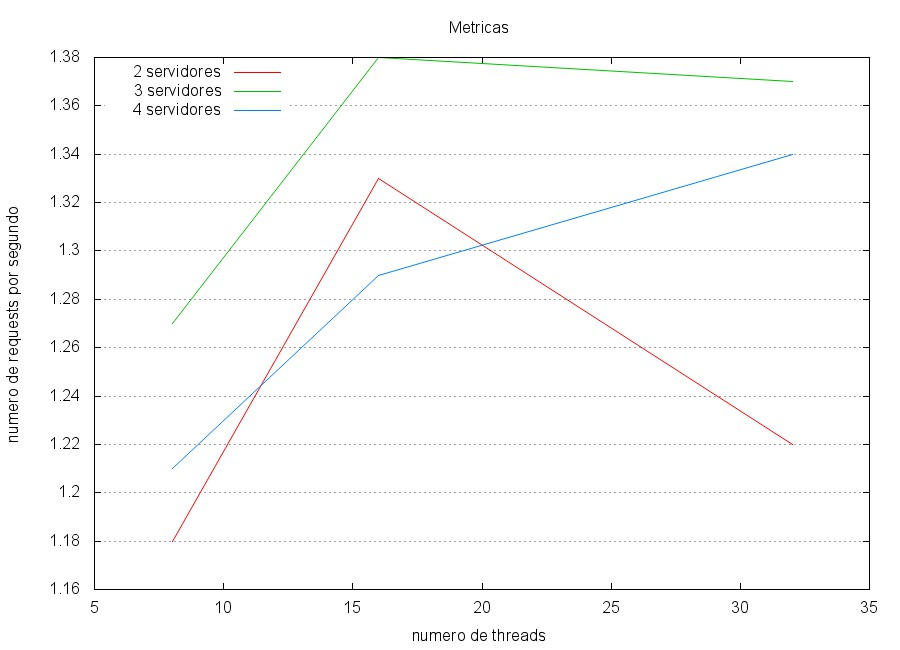
\includegraphics[width=1\textwidth]{images/benchmark/servers}}
\caption{\emph{Benchmark} para dois, três e quatro servidores}
\end{figure}


Como se verifica, a aplicação tem uma grande dificuldade em escalar. O aumento de dois para três servidores aplicacionais resolveu parte do problema, permitindo uma melhoria no desempenho. No entanto, não sendo aquilo que se esperava, adicionar um \emph{Application Server} torna tudo mais lento inicialmente, embora no final do gráfico este continue a crescer. Note, também, que a partir dos 32 clientes o gráfico deixa de existir, devido à falta de recursos para suportar mais do que os referidos. Por acréscimo, as máquinas responsáveis pela \emph{Storage} tiveram um uso de cerca de 30\% de \emph{CPU}.

Tentou-se, também, executar os testes para 64 clientes, mas não se obtiveram resultados, visto que a aplicação atingia o ponto de saturação e o tempo de espera \emph{Apache Bench} alcançava o seu \emph{timeout}.

\section{Conclusões finais}

